\documentclass[a4paper,russian]{article}
\usepackage[utf8]{inputenc}
\usepackage[english,russian]{babel}
\usepackage[14pt]{extsizes}

%\usepackage{pscyr}
\usepackage{subfigure}
\usepackage{wrapfig}
\usepackage{cmap}
\usepackage{indentfirst}
\usepackage{autonum}
\usepackage{amsfonts}
\usepackage{amsmath}
\usepackage{amssymb}
\usepackage{amsthm}
\usepackage{upgreek}
\usepackage{graphicx}
\usepackage{listings}
\usepackage{multirow}
\usepackage{multicol}
\usepackage{dsfont}
\usepackage{graphicx}
\usepackage{caption}
\usepackage{setspace,amsmath}

\usepackage[unicode, pdftex]{hyperref}
\usepackage[left=30mm, top=20mm, right=15mm, bottom=20mm, footskip=10mm]{geometry}

\begin{document}
	\selectlanguage{russian}
\setcounter{page}{0}

\begin{center}
	\small{Министерство науки и высшего образования Российской Федерации}\\
	\small{Федеральное государственное бюджетное образовательное учреждение}\\
	\small{Высшего образования}\\
	\small{\textbf{«Северо-Осетинский государственный университет\\
			имени Коста Левановича Хетагурова»}}\\
	
	\hfill \break
	\hfill \break
	\hfill \break
	\hfill \break
	\hfill \break
	\hfill \break
	\hfill \break
	\hfill \break
	\hfill \break
	\hfill \break
	\hfill \break
	\hfill \break
	\hfill \break
	
	\normalsize{Дипломная работа}\\
	\large{\textbf{Seq2Seq - подход для реализации машинного перевода}}\\
	
	\hfill \break
	\hfill \break
	\hfill \break
	\hfill \break
	\hfill \break
	\hfill\break
\end{center}

\begin{flushright}
	\textbf{Выполнил:}\\
	Студент 4 курса направления:\\
	«Прикладная математика и информатика»\\
	\textit{Гамосов Cтанислав Станиславович \underline{\hspace{3cm}}}\\
\end{flushright}

\hfill

\begin{flushright}
	\textbf{Научный руководитель:}\\
	Кандидат физико-математических наук:\\
	\textit{Басаева Елена Казбековна \underline{\hspace{3cm}}}\\
\end{flushright}

\hfill

\begin{flushright}
	\textbf{Консультант}\\
	Старший преподаватель: \\
	\textit{Макаренко Мария Дмитриевна \underline{\hspace{3cm}}}\\
\end{flushright}

\normalsize{ \hspace{28pt}} \hfill \break
\begin{center} Владикавказ 2022 \end{center}
\thispagestyle{empty}
\clearpage
	\thispagestyle{empty}
\tableofcontents
\thispagestyle{empty}
\clearpage
\newtheorem{theorem}{Теорема}
	
	\section{Введение}
	
	\textbf{Seq2seq} - это семейство подходов машинного обучения, используемых для обработки естественного языка. Основные задачи для которого используется данные методы: нейронный перевод, субтитры к изображениям, разговорные модели и обобщение текста.
	
	Первоначальный алгоритм, который в процессе породил целое семейство методов, был разработан \textit{Google} для использования в машинном переводе. Как уже можно заметить за последнюю пару лет коммерческие системы стали удивительно хороши в  переводе - посмотрите, например, \textit{Google Translate}, \textit{Яндекс}-переводчик, переводчик \textit{DeepL}, переводчик \textit{Bing Microsoft}.
	
	Так же \textbf{Seq2seq} технология несет в себе огромный потенциал, помимо привычного машинного перевода между естественными языками, вполне реализуем перевод между языками программирования (\textit{Facebook AI "Глубокое обучение переводу между языками программирования"}). Поэтому возможности применений такого рода подходов довольно велики. В связи с этим под машинным переводом будет подразумеваться любая задача \textbf{Seq2seq}, если точнее, то перевод между последовательностями любой природы.
	
	\clearpage
	
	\section{Формализация задачи машинного перевода}
	
	Формально в задаче машинного перевода у нас есть входная последовательность $x_{1}, x_{2}, ... x_{m}$ и последовательность вывода $y_{1}, y_{2}, ... y_{n}$, само собой длинна данных последовательностей может отличатся. Саму процедуру \textit{перевода} можно рассматривать как нахождение искомой последовательности, которая является наиболее вероятной с учетом входных данных. Формально искомая последовательность, которая максимизирует условную вероятность $p(y|x): y^{'} = argmax[p(y|x)]$.
	
	Когда человеку известны уже два языка с которыми он работает, то уже при переводе можно сказать насколько хорошо справилась модель, является ли перевод естественным и насколько он приятен на слух. Однако такой вид анализа неприемлем для машины, поэтому нам стоит проанализировать уже имеющуюся функцию $p(y|x,\theta)$ с неким параметром $\theta$, а затем найти его $argmax$ для $y^{'} = argmax_{y}[p(y|x, \theta)]$.
	
	Прежде чем перейти к самой задачи перевода, нужно ответить на 3 вопроса:
	
	\begin{itemize}
		\item \textbf{Моделирование}: Как работает модель для $p(y|x, \theta)$?
		\item \textbf{Обучение}: Как найти параметр $\theta$?
		\item \textbf{Вывод}: Как понять, что текущий $y$ лучший?
	\end{itemize}
	
	\clearpage
	
	\section{Рекуррентные сети}
	
	\subsection{RNN - Recиrrent Neural Network}
	
	Одно из важных отличий RNN от обычных нейронных сетей это понятие времени. Под ним подразумевается последовательность входных данных $x^t$, которые поступают на вход, и их выходные результаты $y^t$, которые генерируются для дискретной последовательности, индексируемых $t$. 
	
	Получаемые последовательности могут быть конечной длины или бесконечно счетными. Таким образом, входную последовательность можно обозначить $x = (x_1, x_2, x_3, ... , x_T)$, а выходную последовательность как $y = (y_1, y_2, y_3, ... , y_T)$
	
	\begin{wrapfigure}{r}{0.25\textwidth}
		\centering
		\captionsetup{justification=centering}
		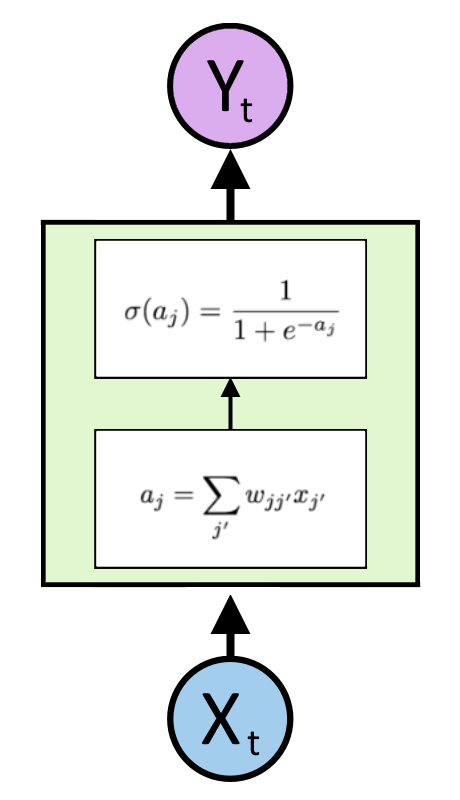
\includegraphics[height=65mm]{img/1.png}
	\end{wrapfigure}
	
	Рекуррентные нейронная сеть как и обычные нейронные сети представляют из себя граф состоящий из набора искусственных нейронов (вершин), обычно называемых \textbf{узлами}, и набора направленных взвешенных ребер между ними. Каждый нейрон $j$ связан \textbf{функцией активации} $\sigma_j$.
	
	\textbf{Вес} - это связь между нейронами, которая несет в себе значение, которое характеризует важность, придаваемая значению сигнала, проходящего через данное ребро или синапс. Для каждого ребра от узла $j'$ до $j$ присутствует вес $w_{jj'}$. Значение $v_j$ каждого нейрона вычисляется путем применения его функции активации к взвешенной сумме его входных данных: 
	
	$$v_j = l_j\bigg(\sum_{j'} w_{jj'} \cdot v_{j'}\bigg)$$
	
	Для удобства обозначим $a_j = \sum_{j'} (w_{jj'} \cdot v_{j'})$ и назавём \textbf{текущей активацией}. 
	
	\textbf{Функция активации} $\sigma(z)$ является абстракцией, представляющей скорость возбуждения нейрона. Обычно в качестве функций активации применяют:
	
	\begin{table}[h]
		\centering
		\begin{tabular}{|l|l|} 
			\hline
			Функция Хевисайда       &   
			$ H(x) = 
			\begin{cases}
				0, & x < 0 \\
				1, & x >= 0 \\
			\end{cases}$ \\ 
			\hline
			Cигмоида                &  $\sigma(x) = \frac{1}{1 + e^{-x}}$ \\ 
			\hline
			Гиперболический тангенс &  $tanh(x) = \frac{e^x - e^{-x}}{e^x + e^{-x}}$ \\ 
			\hline
			Линейный выпрямитель    &  $ReLU(x) = max(0, x)$ \\
			\hline
		\end{tabular}
	\end{table}

	\clearpage
	
	Некоторые желательные свойства функций активации:
	
	\begin{itemize}
		\item \textit{Нелинейность} – Если функция активации нелинейна, то двухуровневая нейронная сеть будет универсальным аппроксиматором функции. Тождественная функция активации не удовлетворяет этому свойству. Если несколько уровней используют тождественную функцию активации, вся сеть эквивалентна одноуровневой модели.
		
		\item \textit{Непрерывная дифференцируемость} – Это свойство желательно (RELU не является непрерывно дифференцируемой и имеет некоторые проблемы с оптимизацией, основанной на градиентном спуске, но остаётся допустимой возможностью) для обеспечения методов оптимизации на основе градиентного спуска.
		
		\item \textit{Область значений} – Если множество значений функции активации ограничено, методы обучения на основе градиента более стабильны, поскольку представления эталонов существенно влияют лишь на ограниченный набор весов связей. Если область значений бесконечна, обучение, как правило, более эффективно, поскольку представления эталонов существенно влияют на большинство весов. В последнем случае обычно необходим меньший темп обучения.
		
		\item \textit{Монотонность} – Если функция активации монотонна, поверхность ошибок, ассоциированная с одноуровневой моделью, гарантированно будет выпуклой.
		
		\item \textit{Гладкие функции с монотонной производной} – Показано, что в некоторых случаях они обеспечивают более высокую степень общности.
		 
		\item \textit{Аппроксимирует тождественную функцию около начала координат} – Если функции активации имеют это свойство, нейронная сеть будет обучаться эффективно, если её веса инициализированы малыми случайными значениями. Если функция активации не аппроксимирует тождество около начала координат, нужно быть осторожным при инициализации весов.
	\end{itemize}
	
	\textbf{Рекуррентные Нейронные Сети (Recиrrent Neural Network - RNN)} - это нелинейная динамическая система, которая сопоставляет последовательности с последовательностями. Основная философия заключается, в том что мысли обладают неким постоянством и напрямую зависят от прошлых умозаключений. Традиционные нейронные сети на такое не способны, и это, очевидно, серьезный изъян. 
	
	Допустим перед нами стоит задача научить сеть определять эмоциональный окрас предложения, и подаём в сеть одно слово за другим. Желательно, чтобы сеть "помнила"\ уже переданные слова. Уже здесь возникает проблема обычных нейронных сетей, как же "запоминать"\ контекст? Если мы хотим, чтобы сеть переводила предложение с одного языка на другой, то тоже было бы не плохо учитывать начало, середину и конец предложение при переводе. В таких случаях именно рекуррентные нейронные сети призванны решить такие проблемы.

	RNN способны работать с последовательностями произвольной длины, а не с входными данными фиксированного размера. Это свойство как раз таки очень важно в контексте обработки естественных языков. 

	\begin{figure}[ht!]
		\centering
		\captionsetup{justification=centering}
		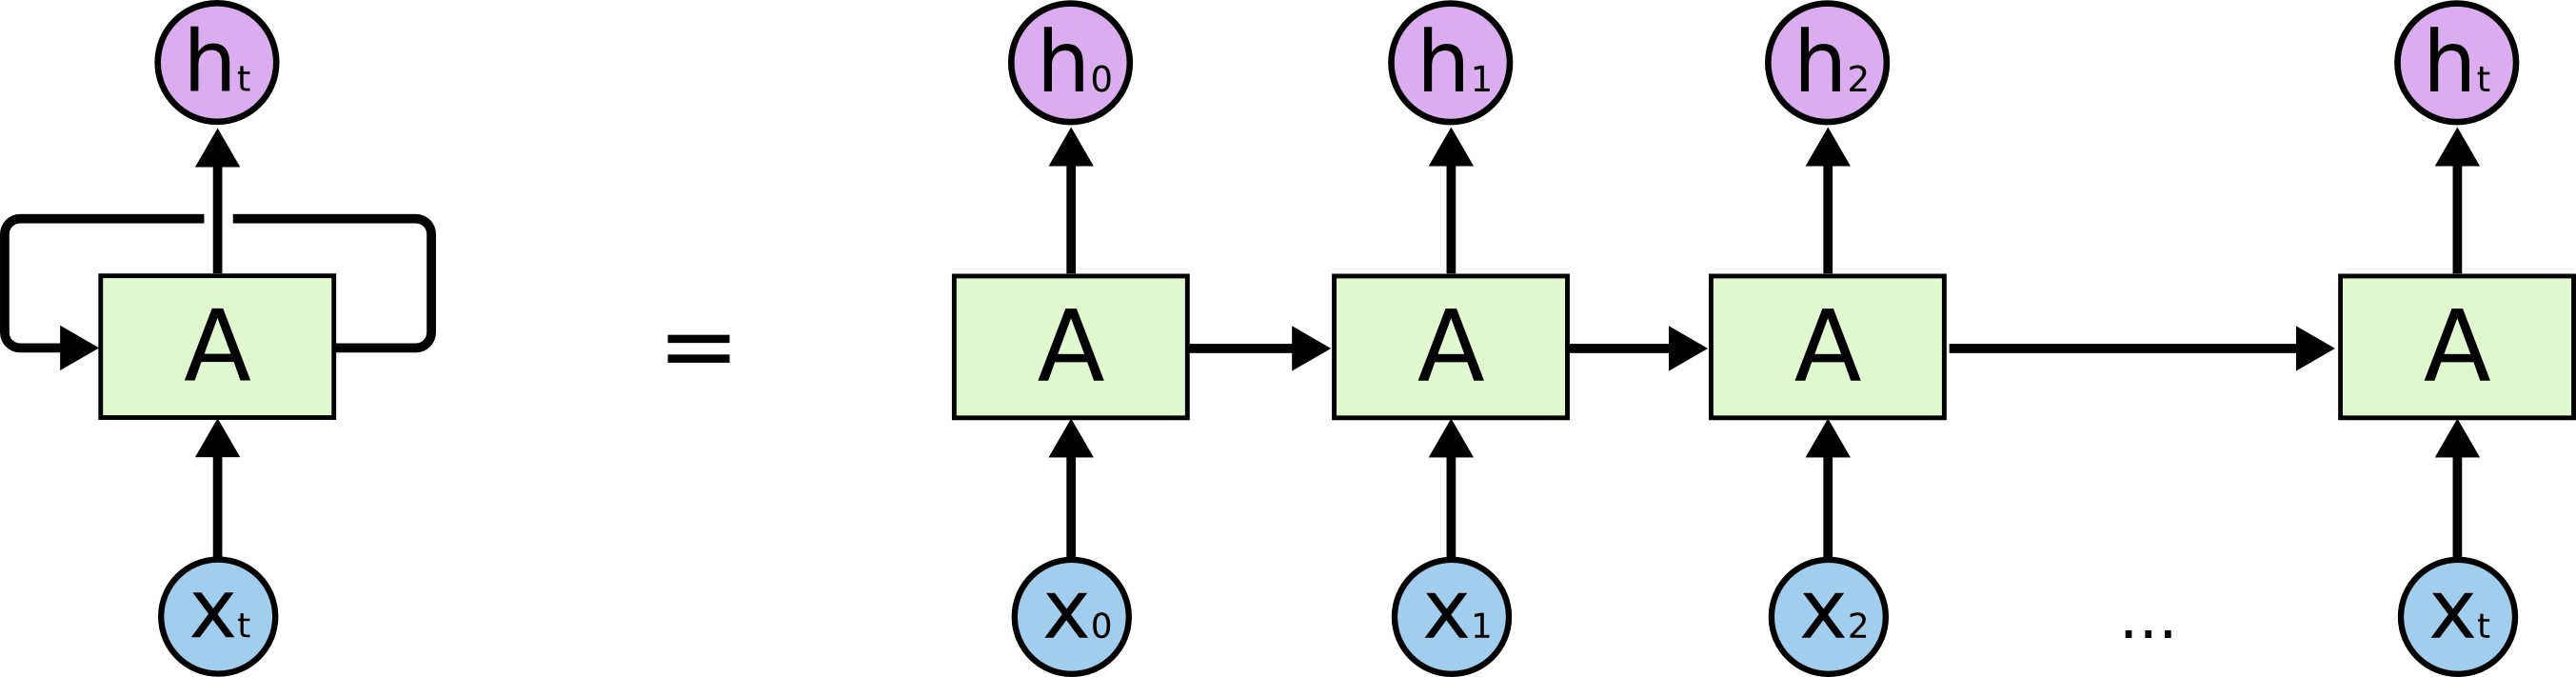
\includegraphics[height=40mm]{img/3.png}
		\caption{Развернутая рекуррентная нейронная сеть}
	\end{figure}
	
	Такая "цепная"\ сущность еще раз показывает, что рекуррентные нейронные сети по природе своей тесно связаны с последовательностями. 
	
	Кроме выходного вектора, где мы будем получать ответ, сеть должна иметь еще и некоторый вектор или векторы в, которых описывает текущее внутреннее состояние сети, т.е. в нем содержатся воспоминания о всех уже отсмотренных сетью элементах. Более формально это выглядит так.
	
	\begin{equation}
		h_t = 
		\begin{cases}
			0 & t = 0 \\
			\sigma(h_{t - 1}, x_t) & \text{в противном случае}
		\end{cases}
	\end{equation}

	где $\sigma$ является нелинейной активации функцией. Необязательно, RNN может иметь выходной сигнал $y = (y_1, y_2, y_3, ... , y_T)$, который может иметь иную длину.
	
	Традиционно обновление скрытого состояния реализуется как:
	
	$$ h_t = \sigma(W x_t + U h_{t-1}) $$
	
	\clearpage
	
	Таким ячейки собираются в последовательность, передавая внутреннее состояние из ячейки в следующую за ней по времени. Отметим, что веса при этом у всех ячеек одни и теже:
	
	\begin{figure}[ht!]
		\centering
		\captionsetup{justification=centering}
		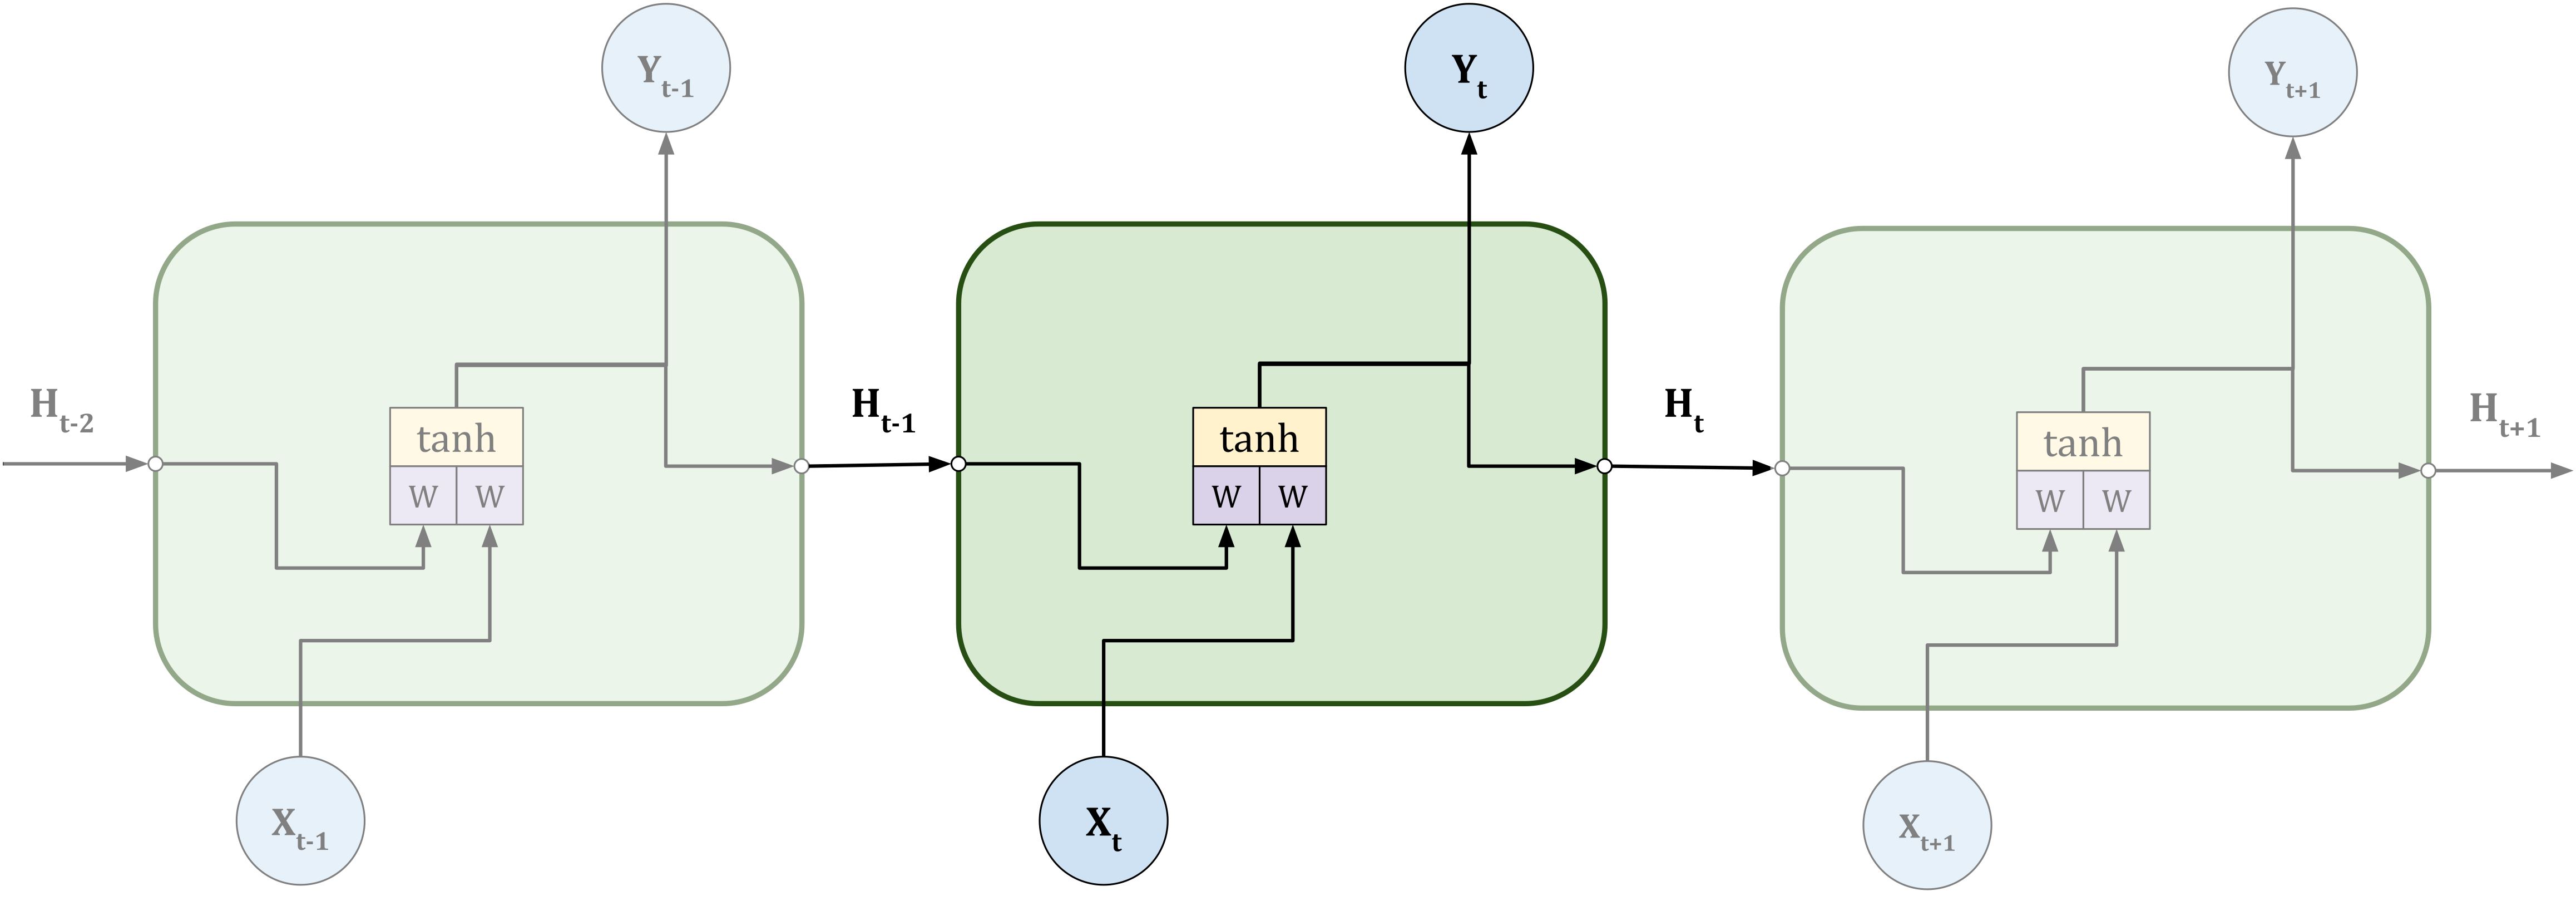
\includegraphics[width=165mm]{img/rnn_unfolded.png}
	\end{figure}
	
	Более формально, учитывая последовательность $x = (x_1, x_2, x_3, ... , x_T)$, RNN обновляет свое скрытое состояние. 
	
	Порождающий RNN выводит распределение вероятности по следующему элементу последовательности, учитывая его текущее состояние ht, и эта порождающая модель может фиксировать распределение по последовательностям переменной длины, используя специальный выходной символ для представления конца последовательности. Вероятность последовательности может быть разложена на:
	
	$$ p(x_1, x_2, ..., x_T) = p(x_1) p(x_2 | x_1) p(x_3 | x_1, x_2) ... p(x_T | x_1, x_2, ... , x_{T - 1}) $$
	
	где последний элемент - это специальное значение конца последовательности. Мы моделируем каждое условное
	распределение вероятностей с помощью:
	
	$$ p(x_t | x_1, x_2, ... , x_{t - 1} = \sigma(h_t)) $$
	
	Существуют несколько конфигураций простых RNN:
	
	\begin{table}[h]
			\centering
			\begin{tabular}{|c|c|} 
				\hline
				\textbf{Elman Networks} & \textbf{Jordan Networks}  \\ 
				\hline
				$	h_{t} = \sigma_{h}(W_h x_t + U_h h_{t - 1} + b_h) $ & 
				$	h_{t} = \sigma_{h}(W_h x_t + U_h y_{t - 1} + b_h) $  \\
				$	y_{t} = \sigma_{y}(W_y h_t + b_y) $ & 
				$	y_{t} = \sigma_{y}(W_y h_t + b_y) $ \\
				\hline
			\end{tabular}
	\end{table}
	
	\begin{tabbing}
		$x_t$ - вектор входного слоя \\
		$h_t$ - вектор срытого слоя \\
		$y_t$ - вектор выходного слоя \\
		$W$, $U$ и $b$ - матрицы и векторы параметров \\
		$\sigma_h$ и $\sigma_t$ - функции активации
	\end{tabbing}
	
	\begin{figure}[ht!]
		\centering
		\captionsetup{justification=centering}
		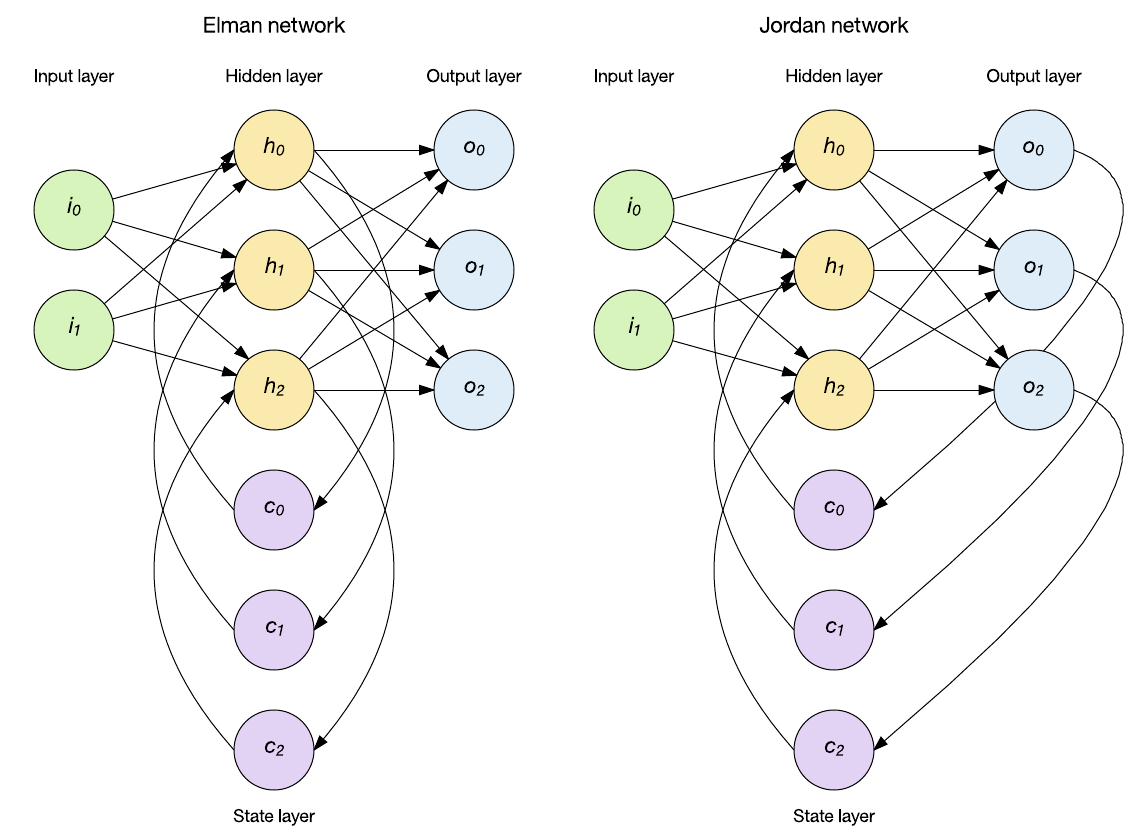
\includegraphics[width=140mm]{img/RNN.png}
	\end{figure}
	
	Во время работы с RNN было замечено, что трудно обучить такие модели. Долгосрочные зависимости плохо воспринимаются обычными рекурсивными сетями, потому что градиенты имеют тенденцию либо исчезать (большую часть времени), либо взрываться (редко, но с серьезными последствиями). Это затрудняет метод оптимизации на основе градиента не только из-за различий в величинах градиента, но и из-за того, что эффект долгосрочных зависимостей скрыт (будучи экспоненциально меньшим по отношению к длине последовательности) эффектом
	краткосрочных зависимостей. 
	
	Существовало два доминирующих подхода, с помощью которых многие исследователи попытались уменьшить негативные последствия этой проблемы. Один из таких подходов заключается в разработке лучшего самообучающийся алгоритм, чем простой стохастический градиентный спуск.
	
	Другой подход, который нас больше интересует, заключается в разработке более сложной функции активации, чем обычные функции что применялись ранее. Самая ранняя попытка в этом направлении привела к появлению функции активации или повторяющегося блока, называемого блоком долговременной кратковременной памяти (LSTM)[1997]. Более современный тип повторяющейся единицы, к которому мы относимся как к закрытой повторяющейся единице (GRU)[2014]. Было показано, что некоторые из этих повторяющихся блоков хорошо справляются с задачами, требующими учета долгосрочных зависимостей.
	
	\clearpage
	
	\subsection{GRNN - Gated Recurrent Neural Networks}
	\subsubsection{LSTM - Long Short-Term Memory}
	
	Сети долгой краткосрочной памяти (LSTM) в отличие от обычных рекуррентных сетей, которые просто вычисляют взвешенную сумму входного сигнала и применяют нелинейную функцию активации, каждый j-й блок LSTM поддерживает память $c^{j}_{t}$ в момент времени $t$. Выходной сигнал $h^{j}_{t}$ или активация, блока LSTM затем
	
	$$h^{j}_{t} = o^{j}_{t} tanh(c^{j}_{t})$$
	
	где $o^{j}_{t}$  - выходной вентиль (\textit{output gate}), который модулирует объем содержимого памяти. Выходной вентиль вычисляется с помощью:
	
	$$ \sigma^{j}_{t} = \sigma(W_{o} x_{t} + U_{o} h_{t - 1} + V_{o} c_{t})^{j}$$
	
	где $\sigma = \frac{1}{1 + e^{-x}}$ - логистическая сигмоидальная функция. $V_{o}$ - это диагональная матрица.
	
	Ячейка памяти $c^{j}_{t}$ обновляется путем частичного удаления существующей памяти и добавления нового содержимого памяти $\overline{c}_{t}^{j}$:
	
	$$ c^{j}_{t} = f^{j}_{t} c^{j}_{t - 1} = i^{j}_{t} \overline{c}_{t}^{j}$$
	
	где находится новое содержимое памяти
	
	$$ \overline{c}_{t}^{j} = tanh(W_{c} x_{t} + U_{c} h_{t - 1})^j $$
	
	Степень, в которой существующая память забывается, модулируется вентилем забывания (\textit{forget gate}) $f^{j}_{t}$, а степень, в которой новое содержимое памяти добавляется в ячейку памяти, модулируется входным вентилем (\textit{inpit gate}) $i^{j}_{t}$. Вентили вычисляются по формула:
	
	$$ f^{j}_{t} = \sigma(W_f x_t = U_f h_{t - 1} + V_f c_{t - 1})^j $$
	$$ i^{j}_{t} = \sigma(W_i x_t = U_i h_{t - 1} + V_i c_{t - 1})^j $$
	
	Обратите внимание, что $V_f$ и $V_i$ являются диагональными матрицами.
	
	В отличие от традиционных рекуррентных сетей, которые перезаписывают свое содержимое на каждом шаге времени, блок LSTM способен решать, следует ли сохранять существующую память или нет с помощью введенных элементов. Интуитивно понятно, что если модуль LSTM обнаруживает важную функцию из входной последовательности на ранней стадии, он легко переносит эту информацию на большие расстояния, следовательно, фиксируя потенциальные зависимости.
	
	\clearpage
	
	\subsubsection{GRU - Gated Recurrent Unit}
	
	Закрытая рекуррентная единица (GRU) была предложена в 2014, чтобы каждая рекуррентная единица
	могла адаптивно фиксировать зависимости разных временных масштабов. Аналогично блоку LSTM, GRU имеет
	вентильные блоки, которые модулируют поток информации внутри блока, однако, не имея отдельных
	ячеек памяти.
	
	Активация слоя $h^{j}_{t}$ GRU в момент времени $t$ представляет собой линейную интерполяцию между предыдущей активацией $h^{j}_{t}$ и возможной активацией $\overline{h}^{j}_{t}$:
	
	$$ h^{j}_{t} = (1 - z^{j}_{t})h^{j}_{t - 1} + z^{j}_{t} \overline{h}^{j}_{t} $$
	
	где вентиль обновления $z^{j}_{t}$ решает, насколько устройство обновляет свою активацию или содержимое. Вентиль обновления вычисляется по формуле:
	
 	$$ z^{j}_{t} = \sigma(W_z x_t + U_z h_{t - 1})^j $$

	Эта процедура получения линейной суммы между существующим состоянием и вновь вычисленным состоянием аналогична единице LSTM. GRU, однако, не имеет какого-либо механизма для контроля степени раскрытия своего состояния, но каждый раз раскрывает все состояние целиком.
	
	Потенциальная активация слоя $\overline{h}^{j}_{t}$ вычисляется аналогично как в традиционной рекуррентной сети:
	
	$$ \overline{h}^{j}_{t} = tanh(W x_t + U(r_t \odot h_{t - 1}))^j $$
	
	где $r_t$ - набор вентилей сброса, а $\odot$ - поэлементное умножение. Когда выключено ($r^{j}_{t}$ близко к 0), элемент сброса эффективно заставляет устройство действовать так, как если бы оно считывало первый символ входной последовательности, позволяя ему забыть ранее вычисленное состояние.
	
	Вентиль сброса $r^{j}_{t}$ вычисляется аналогично элементу обновления:
	
	$$ r^{j}_{t} = \sigma(W_r x_t + U_r h_{t - 1})^j $$
	
 	\clearpage
	
	\section{Структура Encoder-Decoder}
	
	Наиболее распространенная модель \textbf{Sequence-to-sequence (seq2seq}) являются модель \textbf{Encoder-Decoder}, в которой обычно используют \textbf{рекуррентную нейронную сеть} (\textbf{RNN}) для кодирования исходной последовательности в один вектор.
	
	На самом деле полученный вектор можно представить как набор образов сущностей с образами взаимоотношений между ними. Этот вектор затем декодируется вторым \textbf{RNN}, который учится выводить выходное предложение, генерируя его по одному слову за раз.
	
	\clearpage
	
	\section{Сбор данных}
	
	Краеугольным камнем в машинном обучении является качество данных. В нашем случае выходной результат, буквально, в большей степени зависит от количества и качества данных.
	
	В работе было применено несколько дата-сетов для проверки реализации модели машинного перевода.
	
	\begin{enumerate}
		\item $rus-eng.txt$ - Дата-сет предложений с переводом с русского языка на английский.
		\begin{enumerate}
			\item Полностью взят с базы данных: \url{https://tatoeba.org/ru/downloads} Кол-во предложений: 621481
		\end{enumerate}
		\item $rus-oss.txt$ - Дата-сет предложений с переводом с русского языка на осетинский.
		Кусочно собран с разных ресурсов, таких как:
		\begin{enumerate}
			 \item Проект \textit{Tatoeba} — обширная база данных предложений и их переводов, постоянно пополняющаяся усилиями тясяч добровольных участников. \url{https://tatoeba.org/ru/downloads}
 		\end{enumerate}
	\end{enumerate}
\end{document}